\documentclass{standalone}
\usepackage{tikz}
\begin{document}
    
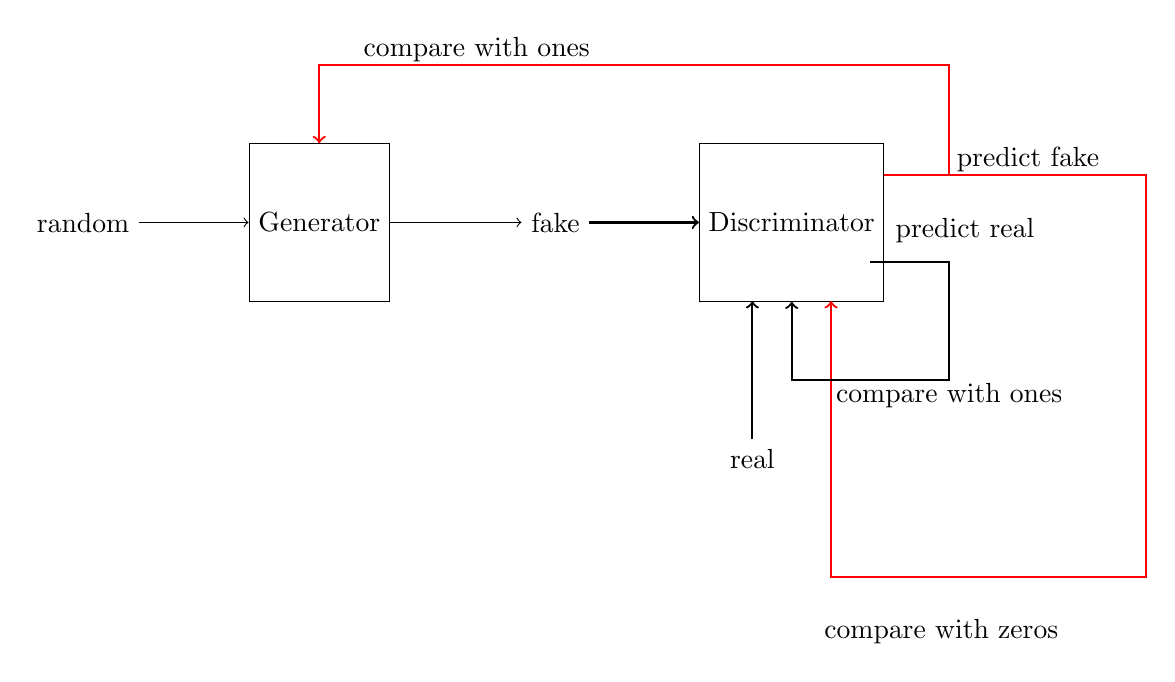
\begin{tikzpicture}
    \path (-3,0) node(start) {random};
    \path (0,0) node(G)[draw,minimum height=2cm] {Generator};
    \path (start) edge[draw,->] (G);
    \path (3,0) node(Gout) {fake};
    \path (G) edge[draw,->] (Gout);
    \path (6,0) node(D)[draw,minimum height=2cm] {Discriminator};
    \path (Gout) edge[draw,->,thick] (D);
    \path (5.5,-3) node(real) {real};
    \path (real) edge[draw,->,thick](5.5,-1);
     \path (D.east){}+(0,0.6)-- (8,0.6)  -- (8,2) [draw,color=red,->,thick] --(0,2)--(G.north);
      \path (D.east){}+(0,0.6)-- (10.5,0.6)  -- (10.5,-4.5) [draw,->,color=red,thick] --(6.5,-4.5)--(6.5,-1);
    \path (7.,-0.5)-- (8,-0.5)  -- (8,-2) [draw,->,thick] --(6.,-2)--(D.south);
    \path (2,2.2) node {compare with ones};
    \path (7.9,-5.2) node {compare with zeros};
    \path (8,-2.2) node {compare with ones};
    \path (9,0.8) node {predict fake};
    \path (8.2,-0.1) node {predict real};
    \node at (-3,1) {};
    \node at (2.5,-2) {};
    \end{tikzpicture}
\end{document}
